\begin{chapter}{Preliminaries}
Throughout the text, $k$ will denote a field of characteristic zero.
\begin{section}{The path algebra of a quiver}
A \emph{quiver} is a quadruple $Q=(Q_0, Q_1, s,t)$, where $Q_0$ and $Q_1$ are finite sets whose elements are called \emph{vertices} and \emph{arrows} respectively, and $s,t:Q_1\to Q_0$ are functions that associate to each arrow $\alpha\in Q_1$ its \emph{source} $s(\alpha)\in Q_0$ and its \emph{target} 
$t(\alpha)\in Q_0$. We will usually abbreviate the fact that an arrow $\alpha\in Q_1$ has source $a$ and target $b$ using the notation $\alpha:a\to b$. We will also omit mentioning $s$ and $t$ explicitly when they are clear from context.

One can represent a quiver graphically as an oriented graph allowing loops and multiple arrows between the same pair of vertices. The following are some examples of quivers:
\[
\begin{tikzpicture}[->, node distance=1cm, thick, auto]
\tikzstyle{every node} = [circle, fill=gray!30, minimum size=.5cm]
\tikzset{every loop/.style={looseness=15}}
\node (a) at (0:1) {};
\node (b) at (120:1) {};
\node (c) at (240:1) {};
\path (a) edge [bend right] (b)
(b) edge [bend right] (c)
(c) edge [bend right] (a)
(a) edge [in=15, out=-15, loop] (a)
(b) edge [in=135, out=105, loop] (b)
(c) edge [in=255, out=225, loop] (c);
\node (d) [right=of a,xshift=2cm] {};
\node (e) [right=of d] {};
\foreach \from/\to in {d/e, e/d}
\draw (d.40) -- (e.140);
\draw (e) -- (d);
\draw (d.320) -- (e.220);
\end{tikzpicture}
\]
\[
\begin{tikzpicture}[->,node distance=1cm, thick]
\tikzstyle{every node} = [circle, fill=gray!30, minimum size=.5cm]
\node (1) {};
\node (2) [right=of 1] {};
\node (3) [right=of 2] {};
\node (4) [right=of 3] {};
\node (5) [right=of 4] {};
\node (6) [right=of 5] {};
\node (7) [right=of 6] {};
\node (8) [below=of 3] {};
\foreach \from/\to in {2/1, 3/2, 3/4, 3/8, 4/5, 5/6, 6/7}
\draw [->] (\from) -- (\to);
\end{tikzpicture}
\]
Let $Q=(Q_0, Q_1, s, t)$ be a quiver and consider the $k$-vector spaces $R=k^{Q_0}$ and $A=k^{Q_1}$, which we will call the \emph{vertex span} and \emph{arrow span} of $Q$, respectively. The space $R$ is a commutative $k$-algebra with the product given by pointwise multiplication. We can consider an $R$-bimodule structure on $A$ given as follows: if $r\in Q_0$, $\alpha\in Q_1$ then we define $r\alpha = \delta_{r,t(\alpha)} \alpha$ and analogously $\alpha r = \delta_{r, s(\alpha)}\alpha$, and extend the action linearly. A vertex $r$ acts as the identity on the left (right) of an arrow $\alpha$ if the target (source) of $\alpha$ is $r$, and otherwise it acts as zero. The \emph{path algebra} $\kQ$ associated to the quiver $Q$ is the graded tensor algebra
\[
\kQ = \bigoplus_{n=0}^\infty A^{\otimes_R n},
\]
where we set $A^{\otimes_R 0}=R$. For the sake of simplicity we will usually notate $A^{\otimes_R n}$ as $A^n$ and an elementary tensor $\alpha_n\otimes\dots\otimes \alpha_1$ as $\alpha_n\dots\alpha_1$. Notice that a non-zero element of the form $\alpha_n\dots\alpha_1$ consists of a sequence of \emph{concatenable} arrows $\alpha_i$, that is, arrows such that $s(\alpha_{i+1})=t(\alpha_i)$. We will call such an element a \emph{path of length n}. It is worth observing that the collection of all paths of length $n$ form a basis of $A^n$ as a $k$-vector space. Since $Q_0$ is a basis of $A^0=R$, we will refer to elements of $Q_0$ as \emph{paths of length 0}, which we will usually call \emph{trivial} or \emph{stationary} paths. Considering the fact that $Q_0$ and $Q_1$ are in bijection with paths of length 0 and 1 respectively, we will denote the set of paths of length $n$ as $Q_n$ and the set of all paths as $Q_*$. We can now define source and target functions $s,t:Q_*\to Q_0$ as follows: if $u=\alpha_n\dots\alpha_0\in Q_n$ with $n>0$, then $s(u)=s(\alpha_0)$ and $t(u)=t(\alpha_n)$. Otherwise, if $u=r\in Q_0$ then $s(u)=t(u)=r$. One easily checks that if $a,b\in Q_0$, the space spanned by paths with source $a$ and target $b$ is exactly $b\kQ a$.

The path algebra satisfies the following useful universal property:

\begin{prop} Let $Q$ be a quiver and $\Lambda$ be an associative $k$-algebra with unit. Suppose $f_0:Q_0\to \Lambda$, $f_1:Q_1\to\Lambda$ are maps satisfying:
\begin{enumerate}
\item $\sum_{a\in Q_0} f_0(a)=1$.
\item If $a\in Q_0$, then $f_0(a)^2=f_0(a)$.
\item If $a\neq b$, with $a,b\in Q_0$, then $f_0(a)f_0(b)=0$.
\item If $\alpha:a\to b$ is an arrow in $Q_1$, then $f_1(\alpha) = f_0(b) f_1(\alpha) f_0(a)$.
\end{enumerate}
Then, there exists a unique $k$-algebra morphism $f:\kQ\to \Lambda$ extending $f_0$ and $f_1$.
\end{prop}
\begin{proof} For $n\geq 1$, define $f(\alpha_n\dots\alpha_1)=f_1(\alpha_n)\dots f_1(\alpha_0)$ and let $f(r)=f_0(r)$ for $r\in Q_0$. As the set of all paths forms a basis of $\kQ$ as a vector space, this defines a $k$-linear map $f:\kQ\to \Lambda$. Condition 1 guarantees that such a map preserves the unit and conditions 2, 3 and 4 guarantee that it preserves products involving stationary paths. Since by definition $f$ preserves products of paths of positive length, we conclude that $f$ is a $k$-algebra morphism extending $f_0$ and $f_1$. As for uniqueness, consider another extension $g:\kQ\to\Lambda$. Since $g$ is a $k$-algebra morphism, we have that $g(\alpha_n\dots\alpha_1)= g(\alpha_n)\dots g(\alpha_1)= f_1(\alpha_n)\dots f_1(\alpha_1)=f(\alpha_n\dots\alpha_1)$ for $n\geq 1$ and $g(r)=f_0(r)=f(r)$ for all $r\in Q_0$. Thus $g$ agrees with $f$ in a basis, and so $g=f$ as wanted.
\end{proof}
Let us now consider some examples:
\begin{exmp} Let $Q$ be the quiver with vertices $\{1,\dots,n\}$ and no arrows:
\[
\begin{tikzpicture}[node distance=1cm, auto, thick]
\tikzstyle{every node} = [circle, fill=gray!30, minimum size=.5cm, inner sep=.07cm]
\node (1) {1};
\node (2) [right=of 1] {2};
\node (3) [right=of 2] {3};
\node (4) [right=of 3, fill=white] {...};
\node (5) [right=of 4] {n};
\end{tikzpicture}
\]
The path algebra $\kQ$ is then isomorphic to $k^n = ke_1\oplus\dots\oplus ke_n$, where multiplication is given by $e_i e_j = \delta_{i,j} e_i$ and extended linearly.
\end{exmp}

\begin{exmp}\label{one-loop} Let $Q$ be the quiver with a single vertex $1$ and a single arrow $\alpha:1\to 1$:
\[
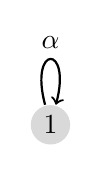
\begin{tikzpicture}[->, thick]
\tikzset{every loop/.style={looseness=15}}
\node[circle, fill=gray!30, minimum size=.5cm, inner sep=.07cm]  (1) {1};
\path (1) edge [loop above] node {$\alpha$} (1);
\end{tikzpicture}
\]
The path algebra $\kQ$ has a basis given by $\{e_1, \alpha, \alpha^2, \dots\}$. It is easily seen that $\kQ$ is isomorphic to the polynomial algebra $k[x]$, via the map sending $\alpha \mapsto x$ and $1\mapsto 1$.
\end{exmp}
\begin{exmp}\label{several-loops} More generally, let $Q$ be the quiver with a single vertex $1$ and $n$ arrows $\alpha_n:1\to 1$:
\[
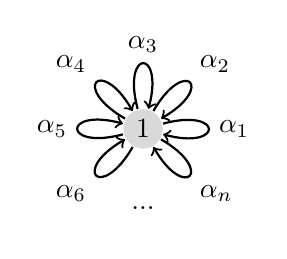
\begin{tikzpicture}[->, auto, thick]
\tikzset{every loop/.style={looseness=15}}
\node[circle, fill=gray!30, minimum size=.5cm, inner sep=.07cm]  (1) {1};
\node[circle, fill=white] (2) at +(270: 1) {...};
\path (1) edge [loop left] node {$\alpha_5$} (1);
\path (1) edge [loop above] node {$\alpha_3$} (1);
\path (1) edge [loop right] node {$\alpha_1$} (1);
\path (1) edge [in=30, out=60, loop] node {$\alpha_2$} (1);
\path (1) edge [in=210, out=240, loop] node {$\alpha_6$} (1);
\path (1) edge [in=120, out=150, loop] node {$\alpha_4$} (1);
\path (1) edge [in=300, out=330, loop] node {$\alpha_n$} (1);
\end{tikzpicture}
\]
The path algebra $\kQ$ is isomorphic to the free algebra on $n$ generators $k\langle x_1,\dots, x_n\rangle$, via the map sending $\alpha_i\mapsto x_i$ and $1\mapsto 1$.
\end{exmp}

A path $u\in Q_n$ with $n>1$ such that $s(u)=t(u)$ is called a \emph{cycle}, and a quiver containing no cycles is said to be \emph{acyclic}. As we can infer from the previous examples, the existence of cycles in the quiver is closely related to the dimension of the path algebra. More precisely, we have:

\begin{prop}\label{acyclic-fin-dim}
Let $Q$ be a quiver and $\kQ$ its associated path algebra. Then $\kQ$ is finite-dimensional iff $Q$ is acyclic.
\end{prop}
\begin{proof} Suppose $\kQ$ is infinite-dimensional. Then the set of all paths $Q_*$, which is a basis for $\kQ$, must be infinite. Since the quiver has only a finite number of arrows, there is only a finite number of paths of less than a fixed length. Therefore, if the set of paths $Q_*$ is infinite, then there exist arbitrarily long paths. Let $n$ be the number of vertices in $Q_0$ and pick a path $\alpha_m\dots\alpha_1$ with $m>n$. Then $s(\alpha_i) = t(\alpha_j)$ for some $1\leq i < j\leq m$ and so $\alpha_j\dots\alpha_i$ is a cycle in $Q$.

Conversely, if $Q$ contains a cycle $u$, then $\{u,u^2,u^3,\dots\}$ is an infinite linearly independent set, and so $\kQ$ is infinite-dimensional.
\end{proof}
\end{section}

\begin{section}{Completions}
In this section we will outline the construction of the completion of a path algebra. For a more detailed treatment of this subject, the reader may consult \cite{SAV15}.

Given a quiver $Q$, the path algebra $\kQ$ admits a $k$-algebra norm $\vert \cdot \vert$ such that for each non-zero $x=\sum_{u\in Q_*} \lambda_u u$ we have $\vert x\vert = e^{-\nu(x)}$, where $\nu(x) = \min\{ i\in \NN_0 : |u| = i \text{ and } \lambda_u \neq 0 \}$. In fact, this is not just a norm but an \emph{ultranorm}, which means we have a stronger triangle inequality, namely \[|x+y|\leq \max\{|x|,|y|\}.\] This ultranorm plays nicely with multiplication as well, since \[|xy|=e^{-\nu(xy)}=e^{-\nu(x)-\nu(y)} = e^{-\nu(x)}e^{-\nu(y)}=|x|\cdot|y|.\]

It is thus straightforward to check that the $k$-algebra operations of $\kQ$ are continuous in the topology induced by this ultranorm. These operations extend to the completion of $\kQ$ as a metric space, making it a $k$-algebra itself, which we will call the \emph{complete path algebra} $\KQ$.

Suppose $(x_n)$ is a Cauchy sequence in $\kQ$. If $x_n=\sum_{u\in Q_*} \lambda_u^n u$, we have that the sequence $(\lambda_u^n)$ is eventually constant, since $|x_n-x_m|<e^{-|u|}$ for big enough $n,m$. Therefore, we may identify the Cauchy sequence $(x_n)$ with its termwise limit $x=\sum_{u\in Q_*} \lambda_u u$, where $\lambda_u$ denotes the constant value the sequence $(\lambda_u^n)$ eventually takes. Notice that the termwise limit $x$ is not necessarily finitely supported. One can now check that $\KQ$ may be identified with the $k$-algebra $\prod_{n=0}^\infty A^n$, where, as before, $A^n$ stands for the $k$-vector spanned by paths of length $n$. The norm $|\cdot|$ extends naturally to this algebra, and it is easy to see that the usual path algebra $\kQ$ is a dense $k$-subalgebra and $R$-subbimodule of $\KQ$.

We now consider the completions of the examples of path algebras mentioned previously:

\begin{exmp}Let $\kQ$ be a finite-dimensional path algebra. Since we must have $A^n=0$ for big enough $n$, we conclude that $\bigoplus A^n=\prod A^n$ and thus the path algebra coincides with its completion. As we proved in \hyperref[acyclic-fin-dim]{Proposition \ref*{acyclic-fin-dim}}, this may only happen if the quiver $Q$ is acyclic.
\end{exmp}

\begin{exmp}Let $Q$ be the quiver from \hyperref[several-loops]{Example \ref*{several-loops}}. The isomorphism $\kQ\simeq k\langle x_1,\dots,x_n\rangle$ extends to an isomorphism between the respective completions $\KQ\simeq k\langle\!\langle x_1,\dots,x_n\rangle\!\rangle$, where the right-hand side term denotes the algebra of non-commutative formal power series in $n$ variables.
\end{exmp}

We end this section with a trivial remark that will be used extensively later:

\begin{obs}\label{arbitrarily-long} Let $I$ be a closed ideal in $\KQ$. Suppose $x$ is a path such that, for all $n\in \NN$, there exists a path $x_n$ of length at least $n$ such that $x=x_n$ in $\KQ/I$. Then, $x=0$ in $\KQ/I$.
\end{obs}
\begin{proof} Let $(x_n)$ be a sequence of paths such that $x=x_n$ in $\KQ/I$ and $x_n$ is of length at least $n$. Then $x-x_n\in I$ and since $|x_n|\leq e^{-n}\to 0$ we have that $x-x_n\to x$. Since the ideal $I$ is closed and the sequence $(x-x_n)$ is contained in $I$, we have that $x\in I$ and therefore $x=0$ in $\KQ/I$.
\end{proof}
\end{section}

\begin{section}{The Jacobian algebra of a quiver with potential}
Let $\KQ=\prod A^n$ be the complete path algebra associated to a quiver $Q$. For $n\geq 1$, we define the \emph{cyclic part} of $A^n$ as
\[
A^n_{\cyc} = \bigoplus_{r\in Q_0} rA^nr,
\]
that is, the $R$-subbimodule spanned by cycles of length $n$. A \emph{potential} $P$ is an element of the closed $R$-subbimodule $\KQ_{\cyc}\subseteq \KQ$, which we define as
\[
\KQ_{\cyc}=\prod_{n=1}^\infty A^n_{\cyc}.
\]
In other words, a potential is a possibly infinitely supported linear combination of cycles. We will call a pair $(Q,P)$ a \emph{quiver with potential}, or \emph{QP} for short.

In their work \cite{RSS80}, Rota, Sagan and Stein introduced a notion of derivative for non-commutative algebras, called the \emph{cyclic derivative}. Here we will work with this concept within the context of the complete path algebra of a quiver. Given an arrow $\alpha\in Q_1$, the cyclic derivative with respect to $\alpha$ is the morphism $\partial_\alpha:\KQ_\cyc\to \KQ$ defined for a cycle $u=\alpha_n\dots\alpha_1$ as
\[
\partial_\alpha(u) = \sum_{k=1}^n \delta_{\alpha, \alpha_k}\alpha_{k+1}\dots\alpha_n\alpha_1\dots\alpha_{k-1}
\]
and extended linearly and continuously.

We are now able to introduce the \emph{Jacobian algebra} associated to a QP, which is the main algebraic object of study in this work. Given a QP $(Q,P)$, the \emph{Jacobian ideal} $J(P)$ is the \emph{closed} ideal in $\KQ$ generated by the set of all cyclic derivatives of the potential, that is, $\{\partial_\alpha(P) : \alpha\in Q_1\}$. The Jacobian algebra $J(Q,P)$ is then the quotient $\KQ/J(P)$.

\begin{exmp} As in \hyperref[one-loop]{Example \ref*{one-loop}}, consider the quiver $Q$ with a single vertex and a unique arrow from that vertex to itself. As we have seen, the complete path algebra $\KQ$ is isomorphic to the algebra of formal power series $k\llbracket x\rrbracket$. Identifying $x$ with the only arrow in the quiver, we see that any potential for Q is of the form $\sum_{n=1}^\infty \lambda_n x^n$ for some choice of scalars $\lambda_n\in k$. For example, let us consider the potential $P=x^n$. Since $x$ is the only arrow in the quiver, we just have to compute $\partial_x(x^n)$, which turns out to be $nx^{n-1}$ (happily coinciding with the usual, commutative notion of derivation). Therefore, the Jacobian algebra is $k\llbracket x\rrbracket/(nx^{n-1})$, which is isomorphic to the truncated polynomial algebra $k[x]/(x^{n-1})$.
\end{exmp}

A direct computation shows that cyclic derivatives vanish on the subspace $V$ of $\KQ_\cyc$ generated by all commutators. Suppose now that $P$ and $P'$ are two potentials. If every term of $P$ is a cyclic permutation of the factors of a term of $P'$ then the difference $P-P'$ lies in $V$ and so $\partial_\alpha(P-P')$ vanishes for any arrow $\alpha$. This in turn implies that $P$ and $P'$ induce both the same Jacobian ideal and the same Jacobian algebra. In this case, we will say that $P$ and $P'$ are \emph{cyclically equivalent}.

\begin{exmp} Let $Q$ be the quiver with vertices 1 and 2, and arrows $\alpha:1\to 2$, $\beta:2\to1$:
\[
\begin{tikzpicture}[->,node distance=1cm, thick]
\tikzstyle{every node} = [circle, fill=gray!30, minimum size=.5cm, inner sep=.07cm]
\node (1) {1};
\node (2) [right=of 1] {2};
\foreach \from/\to in {2/1, 1/2}
\draw (1.20) -- (2.160) node[midway, above, fill=white] {$\alpha$};
\draw (2.200) -- (1.340) node[midway, below, fill=white] {$\beta$};
\end{tikzpicture}
\]
Any potential for $Q$ is of the form $\sum_{n=1}^\infty \lambda_n (\alpha\beta)^n + \mu_n (\beta\alpha)^n$ for some scalars $\lambda_n, \mu_n\in k$. For instance, the cyclically equivalent potentials $P=(\alpha\beta)^n$ and $P'=(\beta\alpha)^n$ give rise to the same Jacobian ideal, which is $(\partial_\alpha(P), \partial_\beta(P)) = (n(\beta\alpha)^{n-1}\beta, n(\alpha\beta)^{n-1}\alpha)$. As any path of length at least $n$ has either $(\beta\alpha)^{n-1}\beta$ or $(\alpha\beta)^{n-1}\alpha$ as factors, the Jacobian ideal contains $A^d$ for $d\geq n$. Therefore, the Jacobian algebra $J(Q,P)$ turns out to be finite-dimensional.
\end{exmp}

In the context of Jacobian algebras, having finite dimension is a highly desirable attribute. A usual method for proving this, as seen in the works of \cites{LF09, Lad12, TVD12}, consists in showing that enough cycles are contained in the Jacobian ideal, just as we did in the toy example above. We will make use of the diamond lemma in order to produce this kind of arguments in a streamlined fashion.
\end{section}

\begin{section}{Ideal triangulations of surfaces}
In this thesis we will focus primarily on a family of QPs (and their associated Jacobian algebras) arising from a particular procedure carried out on a triangulation of a Riemann surface, as described in \cite{LF09}. In order to do this, we start with some basic definitions regarding our geometric objects.

Throughout the text, we will refer to compact, connected, oriented Riemann surface with boundary simply as \emph{surfaces}. We now state a classical result in combinatorial topology that completely classifies these objects:

\begin{prop}\label{surf-classification} Let $\Sigma$ be a surface with a number $b$ of boundary components. Then $\Sigma$ is homeomorphic to either a sphere with $b$ open disks removed or to a $g$-holed torus with $b$ open disks removed.
\end{prop}
\begin{proof} See \cite{Mas77}*{Section 10}.
\end{proof}

The number $g$ appearing in the statement of the previous theorem is called the \emph{genus} of the surface, which we will set as $g=0$ in the spherical case.

A \emph{surface with marked points} $(\Sigma,M)$ is an ordered pair consisting of a surface $\Sigma$ and a finite, non-empty collection $M$ of points (called \emph{marked points}) of $\Sigma$ containing at least one point from each of its boundary components. Points in $M$ that belong to the interior of $\Sigma$ are called \emph{punctures}.

An \emph{arc} on a surface with marked points $(\Sigma, M)$ is a curve $\gamma:[0,1]\to \Sigma$ such that:
\begin{enumerate}
\item Its endpoints lie in $M$.
\item Its restriction to $(0,1)$ is injective and does not intersect $M$ or the boundary of $\Sigma$.
\item Its image is not contractible into $M$ or onto the boundary of $\Sigma$.
\end{enumerate}
\begin{figure}[h]
\[
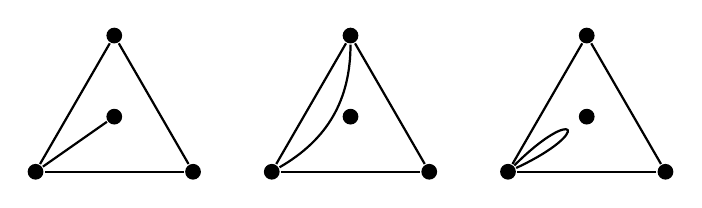
\begin{tikzpicture}[thick]
\tikzstyle{every node} = [circle, fill=black, minimum size=.2cm, inner sep=0cm]
\node (se1) at (0,0) {};
\node (sw1) at (2,0) {}
	edge (se1);
\node (n1) at (1,1.73) {}
	edge (se1)
	edge (sw1);
\node (c1) at (1,0.7) {}
	edge (se1);

\node (se2) at (3,0) {};
\node (sw2) at (5,0) {}
	edge (se2);
\node (n2) at (4,1.73) {}
	edge (se2)
	edge (sw2)
	edge [bend left] (se2);
\node (c2) at (4,0.7) {};

\node (se3) at (6,0) {}
	edge [in=25, out=45, distance=1.1cm] (se3);
\node (sw3) at (8,0) {}
	edge (se3);
\node (n3) at (7,1.73) {}
	edge (se3)
	edge (sw3);
\node (c3) at (7,0.7) {};
\end{tikzpicture}
\]
\caption{While the first is an arc of the punctured triangle, the last two are not, since they are contractible to the boundary or to the set of marked points, respectively.}
\end{figure}

We will consider arcs on a surface only up to isotopy relative to $M$. Two arcs will be said to be \emph{compatible} if there exist representatives in their corresponding relative isotopy classes such that they do not intersect in the interior of $\Sigma$. An \emph{ideal triangulation} for $(\Sigma, M)$ is then a maximal family of compatible arcs in $\Sigma$.

\begin{figure}[h]
\[
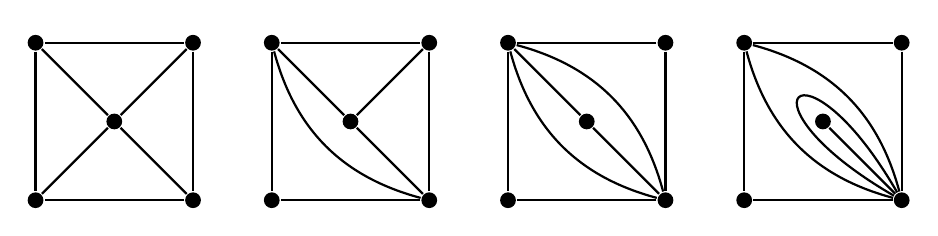
\begin{tikzpicture}[thick]
\tikzstyle{every node} = [circle, fill=black, minimum size=.2cm, inner sep=0cm]
\node (sw1) at (0,0) {};
\node (nw1) at (0,2) {}
	edge (sw1);
\node (se1) at (2,0) {}
	edge (sw1);
\node (ne1) at (2,2) {}
	edge (nw1)
	edge (se1);
\node (c1) at (1,1) {}
	edge (sw1)
	edge (nw1)
	edge (se1)
	edge (ne1);

\node (sw2) at (3,0) {};
\node (nw2) at (3,2) {}
	edge (sw2);
\node (se2) at (5,0) {}
	edge (sw2)
	edge [bend left] (nw2);
\node (ne2) at (5,2) {}
	edge (nw2)
	edge (se2);
\node (c2) at (4,1) {}
	edge (nw2)
	edge (se2)
	edge (ne2);

\node (sw3) at (6,0) {};
\node (nw3) at (6,2) {}
	edge (sw3);
\node (se3) at (8,0) {}
	edge (sw3)
	edge [bend left] (nw3)
	edge [bend right] (nw3);
\node (ne3) at (8,2) {}
	edge (nw3)
	edge (se3);
\node (c3) at (7,1) {}
	edge (nw3)
	edge (se3);

\node (sw4) at (9,0) {};
\node (nw4) at (9,2) {}
	edge (sw4);
\node (se4) at (11,0) {}
	edge (sw4)
	edge [bend left] (nw4)
	edge [bend right] (nw4)
	edge [in=150, out=120,distance=2.4cm] (se4);
\node (ne4) at (11,2) {}
	edge (nw4)
	edge (se4);
\node (c4) at (10,1) {}
	edge (se4);
\end{tikzpicture}
\]
\caption{Some ideal triangulations of the square with one puncture.}
\label{square-triangs}
\end{figure}

An ideal triangulation divides the surface $\Sigma$ into \emph{ideal triangles}. As we can see in \hyperref[square-triangs]{Figure \ref*{square-triangs}}, such triangulations are more general than the usual ones, since they admit configurations in which two triangles share more than one side. Even more, the three sides of an ideal triangle may not be distinct. In that case we say that the triangle is \emph{self-folded}.
\begin{figure}[h]
\[
\begin{tikzpicture}[thick]
\tikzstyle{every node} = [circle, fill=black, minimum size=.2cm, inner sep=0cm]
\node (se1) at (0,0) {};
\node (sw1) at (2,0) {}
	edge (se1);
\node (n1) at (1,1.73) {}
	edge (se1)
	edge (sw1);
\node (cbase1) at (4,0) {};
\node [draw,circle through=(cbase1), fill=none] at (4,1) {};
\node (cbase2) at (7,0) {};
\node (cmid2) at (7,1) {}
	edge (cbase2);
\node [draw,circle through=(cbase2), fill=none] at (7,1) {};
\end{tikzpicture}
\]
\caption{The three possible kinds of ideal triangles: the usual \emph{triangle} and the self-folded ones, which are the \emph{monogon} and the \emph{digon}.}
\end{figure}

Most surfaces may be triangulated without using self-folded triangles. In fact, we have the following result:

\begin{prop}[{\cite{FST08}*{Proposition 2.13}}]\label{no-self-folds} Let $(\Sigma, M)$ be any surface with marked points different from:
\begin{enumerate}
\item A sphere with one, two or three punctures.
\item An unpunctured or once-punctured monogon.
\item An unpunctured digon.
\item An unpunctured triangle.
\end{enumerate}
Then $(\Sigma, M)$ admits an ideal triangulation involving no self-folded triangles. \hfill\qedsymbol
\end{prop}

As one may observe, every ideal triangulation of the square pictured in \hyperref[square-triangs]{Figure \ref*{square-triangs}} consists of exactly 4 arcs. Indeed, the number of arcs in a triangulation is an invariant of the marked surface. More precisely, we have:

\begin{prop}[{\cite{FST08}*{Proposition 2.10}}] Any ideal triangulation of a surface with marked points $(\Sigma, M)$ involving no self-folded triangles consists of exactly
\[
n=6g+3b+3p+c-6
\]
arcs, where $g$ is the genus of the surface $\Sigma$, $b$ is its number of boundary components, $p$ is the number of punctures and $c$ is the number of marked points lying on the boundary.
\end{prop}
\begin{proof} One can show using the classification theorem \ref{surf-classification} that the Euler characteristic of a surface $\Sigma$ of genus $g$ with $b$ boundary components is
\begin{equation}\label{euler-ch1}
\chi(\Sigma)=2-2g-b
\end{equation}
On the other hand, we can compute the Euler characteristic of the surface regarding an ideal triangulation as a cellular decomposition. Since an ideal triangulation is a maximal collection of compatible arcs, any marked point must be a vertex of the decomposition and so we have $v = c + p$ vertices. As for edges, we have $n$ of them in the interior of the surface and $c$ of them in the boundary, which amounts to $e = n + c$. Finally, we know that each face is triangular, that any edge in the interior of the surface belongs to two different faces, and that edges in the boundary belong to only one face. Therefore, by counting faces we arrive at $3f = 2n+c$. Putting it all together, we get that
\begin{align*}\label{euler-ch2}
\chi(\Sigma)&=v-e+f\\
&=(c+p)-(n+c)+\left(\frac{2}{3}n+\frac{1}{3} c\right)\addtocounter{equation}{1}\tag{\theequation}\\
&=p+\frac{1}{3}(c-n)
\end{align*}
The result now follows by equating \eqref{euler-ch1} and \eqref{euler-ch2} and solving for $n$.
\end{proof}
\end{section}

\begin{section}{The QP associated to an ideal triangulation}\label{qp}
We will now introduce a way to produce a QP out of an ideal triangulation, so one may speak of the Jacobian algebra associated to the triangulation.

Taking \hyperref[no-self-folds]{Proposition \ref*{no-self-folds}} into account, from now on we will restrict ourselves to the case where no self-folded triangles appear. Although there is a general mechanism to produce QPs from arbitrary triangulations, as described in Section 3 from \cite{LF09}, technical difficulties arise when dealing with self-folded triangles.

Let $T$ be an ideal triangulation of a surface with marked points $(\Sigma, M)$. We construct a quiver $Q$ following these steps:
\begin{enumerate}
\item Draw a vertex $v_i$ for each edge $e_i$ in the triangulation $T$ that does not belong to the boundary of $\Sigma$.
\item Draw an arrow between two vertices $v_i, v_j$ if $e_i$ and $e_j$ are edges of the same triangle.
\item Orient all arrows according to the already existing orientation on the surface.
\end{enumerate}

Note that every triangle without edges on the boundary of the surface adds a 3-cycle to the quiver. Consider the set $X$ formed by all of these 3-cyles and all other cycles that circle a puncture, and pick a scalar $\lambda_x$ in the field $k$ for each cycle $x\in X$. We thus define the potential $P$ arising from this choice of scalars as
\[P=\sum_{x\in X} \lambda_x x.\]
Notice that this construction is well defined up to cyclic equivalence. Thus, it makes sense to speak of the Jacobian algebra associated from the QP. From now on, we will only consider the potential formed by setting all scalars $\lambda_x=1$, which we will call \emph{the} potential associated to the triangulation $T$, unless we specify otherwise. Moreover, we will refer to the Jacobian algebra induced by the triangulation as the one that is construced from this specific QP.

\begin{exmp} Consider the following triangulation of the torus with a single puncture:
\[
\begin{tikzpicture}[scale=1.2]
\draw[->-=.5] (-1, -1) to (-1, 1); %left vertical line
\draw[->-=.5](1, -1) to (1, 1); %right vertical line
\draw[->-=.5](-1, 1) to (1, 1); %top horizontal line
\draw[->-=.5] (-1,-1) to (1, -1); %bottom horizontal line
\draw (-1, -1) to (1, 1); %diagonal
\end{tikzpicture}
\]
The puncture is placed at the corners of the square, which are all identified. We follow the steps outlined above to obtain the following configuration:
\[
\begin{tikzpicture}[scale=1.2]
\draw[->-=.5] (-1, -1) to (-1, 1); %left vertical line
\draw[->-=.5](1, -1) to (1, 1); %right vertical line
\draw[->-=.5](-1, 1) to (1, 1); %top horizontal line
\draw[->-=.5] (-1,-1) to (1, -1); %bottom horizontal line
\draw (-1, -1) to (1, 1); %diagonal
\draw[->, red, very thick] (0.1, -0.9) to (0.9, -0.1); %a
\draw[->, red, very thick] (0.9, 0) to (0.1, 0); %b
\draw[->, red, very thick] (0, 0.1) to (0, 0.9); %c
\draw[->, red, very thick] (-0.1, 0.9) to (-0.9, 0.1); %d
\draw[->, red, very thick] (-0.9, 0) to (-0.1, 0); %e
\draw[->, red, very thick] (0, -0.1) to (0, -0.9); %f
\end{tikzpicture}
\]
Keep in mind that, since opposing sides of the square are identified, the two triangles of the triangulation share all of their sides, and so this is actually a quiver with three vertices, which we will draw as:
\[
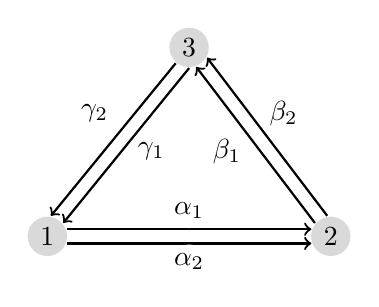
\begin{tikzpicture}[scale=1.2, ->, thick]
\tikzstyle{every node} = [circle, fill=gray!30, minimum size=.5cm, inner sep=.07cm]
\node (1) at (-1.5,0) {1};
\node (2) at (1.5, 0) {2};
\node (3) at (0, 2) {3};
\tikzstyle{every node} = [circle, fill=gray!30, minimum size=.01cm, inner sep=.001cm, fill=white]
\draw (1.20) -- (2.160) node[midway, above] {$\alpha_1$};
\draw  (1.340) -- (2.200) node[midway, below] {$\alpha_2$};
\draw  (2.100) -- (3.330) node at (1,1.3) {$\beta_2$};
\draw  (2.140) -- (3.290) node at (0.4, 0.9) {$\beta_1$};
\draw  (3.270) -- (1.40) node at (-1,1.3) {$\gamma_2$};
\draw  (3.230) -- (1.80) node at (-0.4, 0.9) {$\gamma_1$};
\end{tikzpicture}
\]
Here we have two 3-cycles arising from the two triangles, which are $\gamma_1\beta_1\alpha_1$ and $\gamma_2\beta_2\alpha_2$, and a single 6-cycle that goes around the puncture, which is $\gamma_2\beta_2\alpha_2\gamma_1\beta_1\alpha_1$. Therefore, the associated potential is
\[P = \gamma_1\beta_1\alpha_1+\gamma_2\beta_2\alpha_2+\gamma_2\beta_2\alpha_2\gamma_1\beta_1\alpha_1\]
up to cyclic equivalence.
\end{exmp}
\begin{exmp} Let us now consider a triangulation of a surface with non-empty boundary. The following is a triangulation of the square with a single puncture, placed on its center:
\[
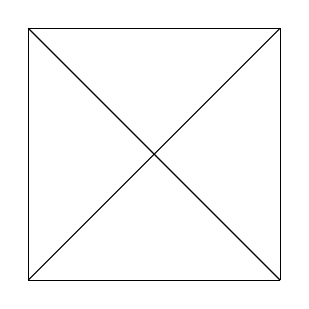
\begin{tikzpicture}[scale=0.8]
\draw (-2,-2) to (-2,2);
\draw (-2,2) to (2,2);
\draw (2,2) to (2,-2);
\draw (2,-2) to (-2,-2);
\draw (-2,-2) to (2,2);
\draw (-2,2) to (2,-2);
\end{tikzpicture}
\]
Every triangle shares an edge with the boundary of the square, so each triangle accounts for only one arrow:
\[
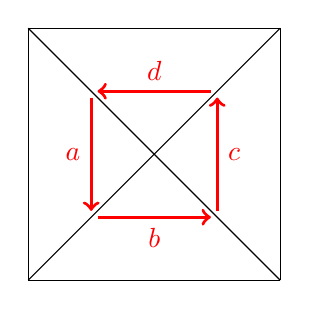
\begin{tikzpicture}[scale=0.8]
\draw (-2,-2) to (-2,2);
\draw (-2,2) to (2,2);
\draw (2,2) to (2,-2);
\draw (2,-2) to (-2,-2);
\draw (-2,-2) to (2,2);
\draw (-2,2) to (2,-2);
\draw[->, red, very thick] (-1,0.9) to node[left] {$a$} (-1, -0.9);
\draw[->, red, very thick] (-0.9,-1) to node[below] {$b$} (0.9, -1);
\draw[->, red, very thick] (1,-0.9) to node[right] {$c$} (1, 0.9);
\draw[->, red, very thick] (0.9, 1) to node[above] {$d$} (-0.9, 1);
\end{tikzpicture}
\]
Since there are no 3-cycles coming from any triangle, the potential $P$ consists simply of the 4-cycle that circles the puncture, which is
\[P=dcba.\]
Notice that we could have chosen $cbad$, $badc$ or $adcb$ as well, since they all define cyclically equivalent potentials.
\end{exmp}
\end{section}
\end{chapter}